\documentclass[11pt]{article}

% packages from hadi's template
\usepackage{bbm}
\usepackage{amsmath}
\usepackage{amssymb}
\usepackage{amsthm}
% \usepackage{chngpage}
\usepackage{fancyhdr}
\usepackage[margin=.7in]{geometry}
\usepackage{graphicx}
\usepackage{hyperref}
% \usepackage{lscape}
\usepackage{mathpazo}
\usepackage{stmaryrd}
% \usepackage{subfigure}
\usepackage{url}

% packages from nam's template
\usepackage{authblk}
\usepackage{amsfonts}
% \usepackage{biblatex}
\usepackage{float}
\usepackage[utf8]{inputenc}
\usepackage{siunitx}
\usepackage{subcaption}
\usepackage[nottoc,numbib]{tocbibind}

% other packages
\usepackage{parskip}

\graphicspath{{figures/}}

\pagestyle{fancy}

\newcommand{\email}[1]{\texttt{\href{mailto:#1}{#1}}}

\lhead{\textbf{Project Report}}
\rhead{\textbf{COMP.4420/5420, UMASS Lowell}}

\def\proptitle{COMP4420 Project Report: Sarcasm Detection in Headlines}
\def\propauthors{Bui, Nam (\#01963609), 
                 Conners, Riley (\#01943861), 
                 Zuk, Sam (\#01642608)}

\begin{document}

\begin{center}
    \textbf{\Large{\proptitle}} \\
    \textbf{\underline{\propauthors}}
\end{center}

\bigskip

\section{Abstract}
% Write a concise summary of the project and the conclusions of the 
% work. It should be no longer than one short paragraph (e.g. 200 
% words).

This project seeks to explore different sentiment analysis techniques in the
task of sarcasm detection in newspaper headlines. We compare the performance of
a Naive Bayes model and LSTM model, with and without pre-trained word2vec
embeddings, on the task. Naive Bayes achieved roughly 80\% accuracy and the
LSTM approaches achieved roughly 90\%. Different embeddings had a negligible
effect on classification, but the switch from a Naive Bayes to an LSTM approach
showed significant improvement.

\section{Introduction}
%Provide an overview of the problem, its significance, potential 
% beneficiaries of its resolution, the challenges associated with 
% its resolution, and a summary of your solution and its results.

Sarcasm is a feature of natural language that is notoriously difficult to
define and identify in both the spoken and written word. It is defined as "the
use of words that convey the opposite meaning to cause or show irritation."
\cite{mw:sarcasm} The assumption that this sarcastic intention will be
recognized is typically contingent upon the listener/reader knowing some
outside piece of contextual information beforehand. However, this external
information isn't always known, and even when it is, the relationship between
it and the statement at hand may not always be clear. When this happens, the
meaning can be obscured as a result, often leading to avoidable scenarios
involving miscommunication.

Recognizing sarcasm typically involves picking up on subtle cues and nuance
that can be difficult to identify. This can often pose a challenge for
populations who encounter greater difficulty when processing certain aspects of
a language. For example, someone trying to interpret a language they don't
speak natively will likely have to expend more mental effort to parse out
meaning from words, which in turn makes it more difficult to pick up on nuance,
including sarcasm. Being unfamiliar with the cultural norms, idioms, etc. that
inform the established meaning of the locally spoken language can also be a
source of confusion. In addition, many neurodivergent people, in particular
those with autism, can struggle to recognize and/or communicate certain social
cues in conversation due to differences between their cognitive experience of
language and what is expected of them.

Finally, there are unique challenges faced in detecting sarcasm in the written
word. It is often possible in practice to infer a statement is sarcastic, even
without necessarily having the context to understand \textit{why} by listening
to changes in the tone of the speaker. However, when translated into the
written word, some or all of this information is lost, making sarcasm even more
difficult to detect when only text is given. With the Internet now being
extremely important to modern infrastructure, and with text being the
predominant medium for online communication, this problem has become
increasingly apparent over the years. This project shall explore and contrast
different approaches to disambiguating sarcasm by applying concepts from the
fields of computational linguistics and machine learning.


\section{Data}\label{sec:data}
% Describe the data used for experiments and report data statistics 
% as well as interesting observations or patterns in the data.

% When and how dataset was collected Headlines collected from The Onion
% (sarcastic) and HuffPost (sincere)
The dataset used for this project is a collection of 28,619 tagged newspaper
headlines -- 13,635 of which originating from the satirical publication
\textit{TheOnion} and the other 14,984 coming from the non-satirical
publication \textit{The Huffington Post} (\textit{HuffPost}). The data was
collected from TheOnion's ``News in Brief'' and ``News in Photos'' sections and
HuffPost's news archive page in 2019 \cite{misra2023Sarcasm}.

% Structure of data in dataset
Each headline is represented as a JSON object with three attributes:
\begin{itemize}
    \item \texttt{is\_sarcastic} (integer): the headline's label -- 1 if
          sarcastic, 0 if not.
    \item \texttt{headline} (string): the text of the headline, case-converted
          to be all lowercase.
    \item \texttt{article\_link} (string): the URL of the referenced article.
\end{itemize}

Our models used the headline text to predict whether or not the article is
sarcastic. Article links were not used by the models themselves, but were
useful in validating the authenticity of the provided headlines. Further
research might find these links useful for the purposes of obtaining and
training on the article text instead of / in addition to the headline alone.

The main limitation of this data collection strategy is its limited scope. It
would be unwise to assume findings on a set of headlines from only two outlets
are representative of the task of sarcasm detection as a whole. Models might
pick up on words and phrases that are less indicative of sarcasm and more
indicative of writing style, formatting guidelines, and/or other details
particular to one source or the other. In addition, since the sort of sarcasm
employed by \textit{TheOnion} tends to be more obvious and outlandish, it's
possible this data may produce models that fail to identify statements that are
sarcastic in subtler ways. 

For example, the two bigrams that occur most frequently amongst
\textit{TheOnion} headlines are [`report', `:'] (427 occurrences) and [`area',
`man'] (231 occurrences). In a headline like "Report: God directly
communicating with you through this headline," sarcasm is conveyed through the
juxtaposition of the formal tone with something later in the text that is
exaggerated, absurd, etc.. It is unlikely that the presence of phrases like
"report:" on their own are indicative of sarcasm; models will need to be able
to pick up on these subtleties in order to be successful.

However, despite the lack of broad generalizability, this data presents a
useful example of a sarcasm detection problem from which meaningful insights
can be gained. Additionally, data collected from reputable media outlets has
advantages over data collected from public social media platforms, which is
often used in sarcasm research.

Since headlines are typically proofread and written in a formal style, their
text tends to contains less slang, fewer spelling and grammar mistakes, and a
lower frequency of very uncommon words. The source-based approach to data
labelling also helps reduce ambiguity about label accuracy, since the sarcastic
intent of a writer at a satire publication is easy to identify.


\section{Method}

% Talk about the manual review of test/validation/training data and manual
% review.
To begin, the dataset described in section \ref{sec:data} was partitioned 70 /
20 / 10 into training / validation / test sets respectively. All articles
labeled as genuine in the test dataset were then manually reviewed to ensure
there were no incorrect labels.

The steps for tokenizing the dataset were:
\begin{enumerate}
    \item Tokenize hyphens.
    \item Tokenize single quotes.
    \item Transform contractions to canonical form.
    \item NLTK word tokenize.
    \item Address edge cases.
\end{enumerate}
The vocabulary included all tokens with $ count > 5 $.

% Naive Bayes
A Naive Bayes model was used to get initial performance baselines.
Along with the tokenized dataset,
lemmatization was used to group words with the same meaning,
like 'says' and 'said', together.
Hyperparameter search was done on the smoothing parameter of the model.
We found that smoothing factor $ \alpha = 1.5 $ performed the best,
although other parameters performed closely.

Word2vec embeddings pre-trained on the Google News dataset
were then fine-tuned over the sarcasm dataset to better fit the dataset. \cite{google-word2vec}
Embeddings for words that were common and unique to the dataset were also added.
Since word2vec does not have an unknown token,
we mapped the unknown token to the 0 vector,
which is what Rishabh and Prahal did in their research. \cite{misra2023Sarcasm}
An LSTM model was then trained with and without the pre-trained embeddings.
The architecture of the LSTM model consisted of
embedding layer, LSTM layer, and a fully-connected feedforward network.
Gradient clipping, early stoppage, batching, dropout,
and learning rate scheduling were used during training.
Results can be found in section \ref{sec:res}.


\section{Results}\label{sec:res}

% - Briefly describe the evaluation approach and metrics.
To compare our results with the results of Rishabh and Prahal,
we measured the accuracy of our models on the test set. \cite{misra2023Sarcasm}
Additionally, since this is a binary classification task,
we also used precision, recall, and F1 metrics.

% - Report performance metrics for the method(s) through Figures or 
% Tables.

\begin{table}[tbh]
    \centering
    \begin{tabular}{|c|c|c|c|c|}
        \hline
        Model              & Accuracy & Precision & Recall & F1    \\
        \hline
        Rishabh and Prahal & 0.897    & N/A       & N/A    & N/A   \\
        Hybrid NN          &          &           &        &       \\
        \hline
        Naive Bayes        & 0.793    & 0.806     & 0.795  & 0.800 \\
        \hline
        Plain LSTM         &          &           &        &       \\
        \hline
        LSTM w/ word2vec   &          &           &        &       \\
        \hline
    \end{tabular}
    \caption{Comparison of model performance.}
    \label{tab:perf}
\end{table}

\begin{figure}[tbh]
    \centering
    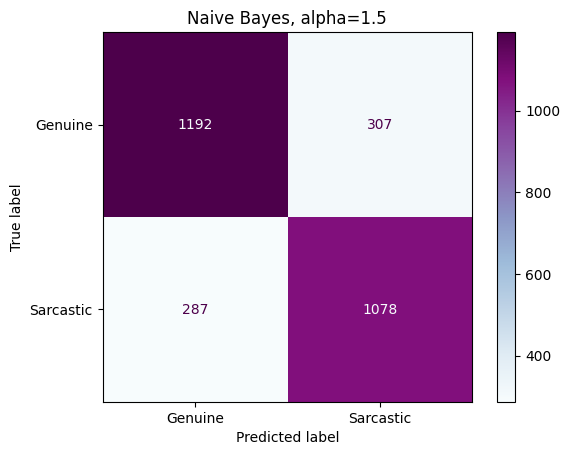
\includegraphics[width=9cm]{nb-cm.png}
    \caption{Confusion matrix of models.}
    \label{fig:cm}
\end{figure}



% - Report insights obtained from the results. Good ways to obtain 
% insight are ablation analysis, error analysis, and use of 
% synthetic data.

The LSTM-based models do not show significant differences in performance.
This implies that the largest factor to performance is the LSTM layer itself.

\section{Conclusion}
% In one short paragraph concisely summarize the main points and 
% insights of the project, describe potential directions to extend 
% your project, and [G] describe limitations of your project.

In conclusion, we found that an LSTM approach outperformed the Naive Bayes.
Sarcasm is a complex concept to identify, especially with only text input.
This project could be extended in the future to work on further
customized dictionaries with word embeddings for new words like Trump.
Customized embeddings for names and/or events could lead to even better
recognition of the meaning behind headlines.
Additionally, it may be useful to include article text in the dataset
so that the model can compare the article text and headline text
because sarcasm comes from a semantic difference between the two.
In terms of the model, an attention layer or stacked LSTM
could also be added to see how it affects performance.

\section{Contribution Chart:}

\begin{table}[H]
    \centering
    \begin{tabular}{c|c|c}
        \hline
        Student Name \& ID          & Tasks/Subtasks                 & Commentary on Contribution   \\
        \hline
        Bui, Nam (\#01963609)       & Tokenized Dictionary           & Created the original files   \\
                                    & Created and Ran Bayes Model    & for both the Bayes and LSTM  \\
                                    & Created LSTM Model             & models, debugged issues with \\
                                    & Debugged Models                & the models, and helped debug \\
                                    &                                & tokenization issues with the \\
                                    &                                & dataset.                     \\
        \hline
        Conners, Riley (\#01943861) & Split Data and Validated Tests & Split the data and manually  \\
                                    & Created Data Loader            & reviewed test set, created   \\
                                    & Ran Initial Runs of LSTM       & the initial dataloader, and  \\
                                    &                                & performed initial            \\
                                    &                                & hyperparameter tuning tests  \\
                                    &                                & with LSTM.                   \\
        \hline
        Zuk, Sam (\#01642608)       & Exploratory Data Analysis      & Conducted the exploratory    \\
                                    & Tokenized Dictionary           & data analysis,               \\
                                    & Created Custom Word Embeddings & helped with tokenizing the   \\
                                    & Ran Final Run of LSTM Model    & the dictionary and creating  \\
                                    &                                & custom word embeddings, and  \\
                                    &                                & created tables on the final  \\
                                    &                                & data on the run of the LSTM. \\
        \hline
    \end{tabular}
    \label{tab:my_label}
\end{table}


\bibliographystyle{plain}
\bibliography{ref}

\end{document}
